% !TeX spellcheck = en_US
% Chapter 2
\chapter{بررسی ادبیات و مبانی نظری}\label{chap:review}

\section{مفاهیم پایه}\label{chap:brain}

\section{مقدمه}

در عصر تحول دیجیتال و صنعت ۵.۰، مفاهیم جدیدی همچون دوقلوهای دیجیتال، عامل‌های هوشمند، سیستم‌های چندعاملی و مدل‌های زبانی بزرگ به عنوان عناصر کلیدی در تحول سامانه‌های هوشمند مطرح شده‌اند. این فصل به بررسی عمیق مبانی نظری این مفاهیم می‌پردازد تا چارچوبی برای پژوهش حاضر فراهم شود \cite{barricelli2019survey,tao2019digital,grieves2017digital}.

% ---------------------------------------
\section{دوقلو دیجیتال}

مفهوم دوقلو دیجیتال نخستین بار توسط \lr{Grieves (2003)} در دانشگاه میشیگان مطرح شد و توسط ناسا برای مأموریت‌های فضایی توسعه یافت \cite{grieves2017digital}. دوقلوی دیجیتال مدلی مجازی از یک موجودیت فیزیکی است که با داده‌های بی‌درنگ در تعامل است و رفتار سیستم واقعی را شبیه‌سازی و پیش‌بینی می‌کند \cite{barricelli2019survey,qi2021digital,jiang2023digital}. 

به طور کلی، یک دوقلوی دیجیتال شامل سه مؤلفه اصلی است:
\begin{enumerate}
	\item \gls{Physical Entity}: تجهیز یا فرایند واقعی که در دنیای فیزیکی قرار دارد.
	\item \gls{Digital Model}: بازنمایی دیجیتال و محاسباتی از موجودیت فیزیکی.
	\item \gls{Data Connection}: مسیر ارتباطی دوطرفه بین مدل و موجودیت برای تبادل داده دو طرفه.
\end{enumerate}

این سه مؤلفه را می‌توان در شکل \ref{fig:dt-structure} مشاهده کرد. همانطور که در شکل مشخص است، یک موجودیت فیزیکی در دنیای واقعی، دارای داده است. این داده‌ها به صورت بی‌درنگ برای دوقلوی دیجیتال خود در دنیای دیجیتال و غیر واقعی ارسال می‌شود. در دنیای دیجیتال امکان تحلیل و بررسی‌های گسترده‌ای روی این داده وجود دارد. پس از انجام این تحلیل‌ و بررسی‌ها، اطلاعاتی فراهم می‌شود که می‌تواند در قالب فرمان‌های مناسب، به موجودیت فیزیکی در دنیای حقیقی، ارسال شود و تغییری روی آن رخ دهد\cite{marah2024madtwin}.

ارتباط بین موجودیت فیزیکی و دیجیتال، می‌تواند با استفاده از حسگرها و اینترنت اشیاء، انجام شود و مدل با استفاده از الگوریتم‌های مختلف \gls{AI} از جمله \gls{ML}، \gls{DL} و \gls{RL}، وضعیت حال را بررسی کرده و رفتار آینده را پیش‌بینی کند.\cite{tao2019digital,liu2024ai}.





\begin{figure}[H]
	\centering
	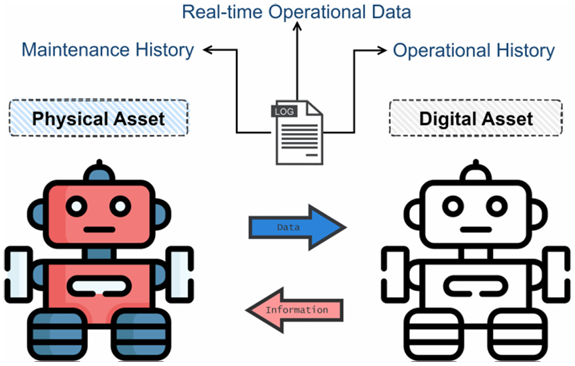
\includegraphics[width=0.85\textwidth]{images/DT_1.png}
	\caption{ساختار مفهومی دوقلوی دیجیتال شامل حلقه داده و اطلاعات بین فضای فیزیکی و فضای دیجیتال \cite{marah2024madtwin}}
	\label{fig:dt-structure}
\end{figure}


\begin{figure}[H]
	\centering
	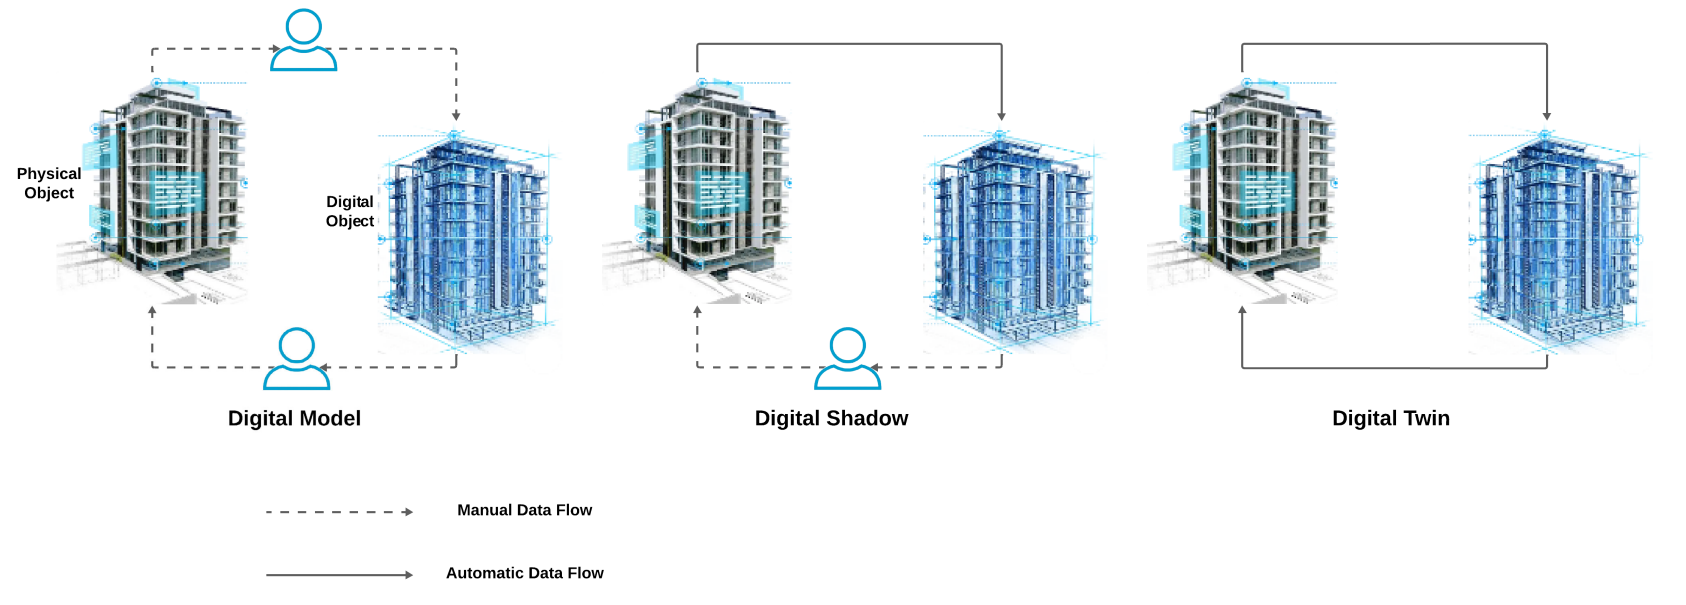
\includegraphics[width=0.85\textwidth]{images/DT_2.png}
	\caption{تفاوت بین \gls{Digital Twins}، \gls{DTSH} و \gls{DTM}\cite{Boukaf2024ComprehensiveReview}}
	\label{fig:dt-types}
\end{figure}


بر اساس مرور جامع پژوهش‌های اخیر، یکی از چالش‌های اساسی در توسعه و پیاده‌سازی دوقلوهای دیجیتال، دشواری در یکپارچه‌سازی کامل تمامی لایه‌ها در یک سامانه‌ی واحد است. این مسئله به دلیل پیچیدگی زیاد در اتصال اجزای فیزیکی، داده‌ای و مجازی، به‌ویژه در سیستم‌های چندعاملی، از اهمیت بالایی برخوردار است \cite{wang2024comprehensive,krizsinger2018digital,grieves2017digital}.

به‌منظور توصیف سطوح مختلف بلوغ و یکپارچگی دوقلوهای دیجیتال، می‌توان آن را بر اساس میزان اتصال میان جهان فیزیکی و دیجیتال، به سه سطح اصلی تقسیم‌بندی کرد\cite{krizsinger2018digital,fuller2020digital}:


\begin{enumerate}
\item 
\gls*{DTM}
در این سطح، ارتباط میان سامانه‌ی فیزیکی و نسخه‌ی مجازی آن به‌صورت دستی انجام می‌شود. داده‌ها از دنیای واقعی به مدل دیجیتال از طریق ورود اطلاعات انسانی منتقل می‌گردند و هیچ‌گونه همگام‌سازی خودکار میان این دو وجود ندارد. هرگونه تغییر در سامانه‌ی فیزیکی باید به‌صورت دستی در مدل دیجیتال اعمال شود. بنابراین، در این سطح هنوز مفهوم واقعی دوقلوی دیجیتال تحقق نیافته است و تنها یک مدل ایستا از سامانه ارائه می‌شود \cite{van2020digital,tao2019digital}.

\item 
\gls*{DTSH}
در این سطح، تعامل میان دنیای فیزیکی و مجازی به‌صورت \lr{یک‌طرفه (Unidirectional)} انجام می‌شود. به این معنا که تغییرات رخ‌داده در سامانه‌ی فیزیکی به‌طور خودکار در مدل دیجیتال بازتاب می‌یابد، اما برعکس آن ممکن نیست. در واقع، اطلاعات از دنیای واقعی به سمت فضای مجازی جریان دارد، اما هیچ تغییری از سوی مدل دیجیتال به دنیای فیزیکی منتقل نمی‌شود \cite{qi2021enabling,barricelli2019survey}.  
این رویکرد در بسیاری از کاربردهای پایش و تحلیل وضعیت تجهیزات رایج است، زیرا به‌سادگی امکان ثبت و نمایش رفتار واقعی را فراهم می‌سازد.

\item 
\gls*{Digital Twins}
در این مرحله، ارتباط \lr{دوطرفه (Bidirectional)} میان دنیای فیزیکی و مدل دیجیتال برقرار است. تغییرات در هر یک از دو حوزه منجر به به‌روزرسانی خودکار دیگری می‌شود. این ساختار موجب می‌شود تا مدل دیجیتال، بازنمایی دقیقی از وضعیت لحظه‌ای، تکامل، و رفتار واقعی سامانه‌ی فیزیکی باشد \cite{tao2018digital,fuller2020digital,wang2024comprehensive}.  
دوقلوی دیجیتال نه‌تنها برای پیش‌بینی خرابی و نگهداری پیش‌بینانه، بلکه برای کنترل، تصمیم‌سازی خودکار، و تعامل بلادرنگ میان انسان و سامانه نیز کاربرد دارد. در واقع، این سطح از بلوغ، نقطه‌ی نهایی در مسیر تحقق دوقلوی دیجیتال محسوب می‌شود که مبنای طراحی چارچوب چندلایه‌ی این پژوهش نیز قرار گرفته است.
\end{enumerate}

 \textbf{مدل دیجیتال (Digital Model)}، \textbf{سایه دیجیتال (Digital Shadow)} و \textbf{دوقلوی دیجیتال (Digital Twin)} .  
این طبقه‌بندی به پژوهشگران کمک می‌کند تا میزان پویایی و هوشمندی تعامل بین اجزای فیزیکی و مجازی را به‌صورت مرحله‌ای ارزیابی کنند.  
نمای کلی این سطوح در شکل \ref{fig:dt_levels} نشان داده شده است.


دوقلوهای دیجیتال تنها یک مدل یا شبیه‌سازی ساده نیست، بلکه یک مدل زنده،‌ هوشمند و در حال تکامل و توسعه است که به عنوان یک همتای مجازی برای موجودیت حقیقی ایجاد می‌شود.




% ---------------------------------------
\section{عامل‌های هوشمند}

عامل هوشمند (\lr{Intelligent Agent}) موجودیتی نرم‌افزاری است که به صورت خودمختار عمل می‌کند، محیط را درک می‌کند و با تصمیم‌گیری مستقل اهداف خود را دنبال می‌کند \cite{wooldridge2009introduction}. 

ویژگی‌های عامل هوشمند عبارت‌اند از:
\begin{itemize}
	\item \textbf{خودمختاری (Autonomy)}: عملکرد بدون کنترل مستقیم انسان.
	\item \textbf{واکنش‌پذیری (Reactivity)}: توانایی پاسخ سریع به تغییرات محیطی.
	\item \textbf{پیش‌فعالی (Proactiveness)}: اقدام آگاهانه برای دستیابی به اهداف.
	\item \textbf{اجتماع‌پذیری (Sociability)}: توانایی تعامل و ارتباط با عامل‌ها و انسان‌ها.
\end{itemize}

مدل‌های کلاسیک \lr{BDI (Belief–Desire–Intention)} از پرکاربردترین چارچوب‌ها برای طراحی عامل‌های هوشمند هستند \cite{rao1995bdi}. اخیراً ترکیب عامل‌های \lr{BDI} با مدل‌های زبانی بزرگ، نسل جدیدی از عامل‌های هوشمند تعاملی را ایجاد کرده است که قادرند از طریق زبان طبیعی دستورات را پردازش و اجرا کنند \cite{li2024llmagent,park2025interactive}.

%\begin{figure}[H]
%	\centering
%	\includegraphics[width=0.75\textwidth]{figures/bdi-agent.png}
%	\caption{معماری عامل هوشمند مبتنی بر مدل BDI \cite{rao1995bdi}}
%	\label{fig:bdi-agent}
%\end{figure}

% ---------------------------------------
\section{سیستم‌های چندعاملی}

سیستم‌های چندعاملی (\lr{Multi-Agent Systems - MAS}) مجموعه‌ای از عامل‌های مستقل هستند که به صورت توزیع‌شده با یکدیگر همکاری می‌کنند تا مسئله‌ای پیچیده را حل کنند \cite{dorri2018multiagent,bellifemine2007jade}. 

مزایای اصلی MAS عبارت‌اند از:
\begin{enumerate}
	\item افزایش مقیاس‌پذیری در مسائل صنعتی.
	\item تصمیم‌گیری غیرمتمرکز و خودمختار.
	\item قابلیت تعامل و مذاکره بین عامل‌ها.
\end{enumerate}

%\begin{figure}[H]
%	\centering
%	\includegraphics[width=0.8\textwidth]{figures/mas-structure.png}
%	\caption{نمای شماتیک ارتباط عامل‌ها در یک سیستم چندعاملی \cite{bellifemine2007jade}}
%	\label{fig:mas-structure}
%\end{figure}

چارچوب‌های نرم‌افزاری مانند \lr{JADE}، \lr{ZEUS} و \lr{SPADE} برای پیاده‌سازی این سیستم‌ها استفاده می‌شوند \cite{bellifemine2007jade,pretel2022masdt}.

% ---------------------------------------
\section{دوقلوهای دیجیتال چندعاملی}

دوقلوهای دیجیتال چندعاملی (\lr{MA-DT}) ترکیبی از دو فناوری MAS و Digital Twin هستند که در آن هر دوقلو دیجیتال به عنوان یک عامل مستقل در محیط دیجیتال عمل می‌کند \cite{pretel2022masdt,wang2024multiagent}. این معماری به سیستم‌ها اجازه می‌دهد تا با تقسیم وظایف بین عامل‌های تخصصی، کارایی و سرعت تصمیم‌گیری را افزایش دهند.

%\begin{figure}[H]
%	\centering
%	\includegraphics[width=0.85\textwidth]{figures/madt-architecture.png}
%	\caption{نمونه‌ای از معماری دوقلوی دیجیتال چندعاملی در سامانه‌های صنعتی \cite{wang2024multiagent}}
%	\label{fig:madt-architecture}
%\end{figure}

در پژوهش‌های اخیر، از دوقلوهای چندعاملی برای پایش زنجیره تأمین، انرژی هوشمند و خطوط تولید استفاده شده است \cite{liu2024ai,he2024mas}. 

% ---------------


\section{مقدمه}

در عصر تحول دیجیتال و گذار به صنعت ۵٫۰، مفاهیمی چون \gls{Digital Twins}، \glspl{MAS}، هوش مصنوعی، و مدل‌های زبانی بزرگ به عناصر کلیدی در تحول سامانه‌های هوشمند تبدیل شده‌اند. در این فصل، هر یک از این مفاهیم به‌صورت مفصل بررسی می‌شوند تا پایه‌ای نظری برای معماری پژوهش حاضر فراهم گردد.

\section{دوقلوی دیجیتال}

دوقلوی دیجیتال به عنوان یک فناوری نوین در حوزه مهندسی و مدیریت سیستم‌ها، از جمله تحولات مؤثر در عصر فناوری اطلاعات محسوب می‌شود. این مفهوم بیشتر در زمینه \glspl{PLM}
مورد توجه قرار گرفته است. 
در واقع، دوقلوهای دیجتیال به معنای وجود یک مدل مجازی وابسته به یک شیء فیزیکی در دنیای واقعی است که از طریق تبادل داده‌ها، همگام‌سازی و تجزیه و تحلیل آنچه در دنیای واقعی اتفاق می‌افتد، امکان بهینه‌سازی عملیات و پیش‌بینی مشکلات را فراهم می‌سازند. یک دوقلوی دیجیتال می‌تواند به روش‌های مختلفی با همتای حقیقی خود ارتباط برقرار کند و بر روی آن اثر گذاشته یا از آن اثر پذیرد.

دوقلوی دیجیتال به عنوان یک پیوند مؤثر میان دنیای فیزیکی و مجازی شناخته می‌شوند که نه تنها تبادل داده‌ را تسهیل می‌کند، بلکه بر پایه آن، امکان تعامل بلادرنگ و بهینه‌سازی فرآیندها را نیز ایجاد می‌کند.
\cite{b2}
این مفهوم از طریق ایجاد یک اتصال دائمی و دوره‌ای بین فضای واقعی و مجازی به وجود می‌آید که در آن، داده‌های دنیای واقعی به فضای مجازی منتقل می‌شوند و برعکس. 
از این رو، دوقلوی دیجیتال می‌تواند حاوی اطلاعات دقیقی از وضعیت فعلی و پیش‌بینی‌های مربوط به شرایط آینده یک سیستم باشد.

می‌توان دوقلوی دیجیتال را به سه بخش اصلی تقسیم کرد:
\cite{b2}
\begin{enumerate}
	\item 
	بخش اول، بخش مجازی که در یک فضای مجازی نیز قرار دارد.
	\item 
	بخش دوم، بخش واقعی و حقیقی که در یک فضای حقیقی و واقعی قرار دارد.
	\item 
	بخش سوم، جریان داده‌ها میان بخش واقعی و بخش حقیقی وجود دارد.
\end{enumerate}

در واقع دوقلوی دیجیتال به مجموعه‌ای از مدل‌‌ها و ماشین‌های فیزیکی یا مجازی گفته می‌شود که عملکرد و چرخه حیات یک موجودیت فیزیکی، را شبیه‌سازی\LTRfootnote{simulating}، تقلید\LTRfootnote{emulating} کرده یا آینه‌وار\LTRfootnote{mirroring} نمایش می‌دهند. البته این دوقلو تنها به موجودیت‌های فیزیکی خلاصه نمی‌شود و می‌توان در لایه‌های مختلفی دوقلو‌های دیجیتال را بررسی کرد:
\begin{itemize}
	\item 
	دوقلوی دیجیتال در سطح اشیاء که در آن سعی بر مجازی‌سازی و ایجاد دوقلوی مجازی از اشیاء و موجودیت‌های مختلف است.
	\item 
	دوقلوی دیجیتال در سطح فرایند که از مجموعه‌ای از کنش‌ و برهم‌ کنش موجودیت‌های مختلف ایجاد می‌شود.
	\item 
	دوقلوی دیجیتال سامانه که از مجموعه‌ای از فرایند‌ها ایجاد می‌شود و قابلیت تعریف و تفسیر سامانه‌ها را دارد.
\end{itemize}

علاوه‌بر انواع مختلفی از دوقلو‌های دیجیتال که به آن‌ها اشاره شد، می‌توان موارد دیگری را نیز در نظر گرفت که با ترکیب کردن آن‌ها، قدرت ایجاد دوقلو‌های دیجیتال بزرگ‌تر، جامع‌تر و کامل‌تری را به صورت قابل توجهی افزایش می‌دهد به طوری که بتوان دوقلو‌های دیجیتال یک انسان یا ویژگی‌های آن‌را نیز ایجاد نمود.

دوقلوهای دیجیتال تنها یک مدل یا شبیه‌سازی ساده نیست، بلکه یک مدل زنده،‌ هوشمند و در حال تکامل و توسعه است که به عنوان یک همتای مجازی برای موجودیت حقیقی ایجاد می‌شود.

\section{عامل}

به طور کلی برای 
\textit{عامل}
یک تعریف واحد و یکتا که در همه زمینه‌ها کاربرد داشته باشد، یافت نمی‌شود. این موضوع به این دلیل است که در زمینه‌های مختلف، می‌تواند ویژگی‌های مختلفی داشته باشد و همچنین اشکال فیزیکی و غیر فیزیکی متنوعی را می‌تواند شامل شود، از ربات‌ها گرفته تا شبکه‌های کامپیوتر و حتی عامل‌های نرم‌افزاری.
یکی از تعاریفی که در حوزه هوش‌مصنوعی ارائه شده به صورت زیر است:

\textit{
	یک برنامه نرم افزاری است که می تواند با محیط خود تعامل داشته باشد، داده ها را جمع آوری کند و از داده ها برای انجام وظایف خود و تصمیم‌گیری در جهت رسیدن به اهداف از پیش تعیین شده استفاده کند.}
\cite{b4}

در برخی‌ از منابع، ویژگی‌های زیر برای یک عامل در نظر گرفته شده است:
\cite{b5}


\begin{description}
	\item[$\bullet$ قرارگیری\footnotemark:] \footnotetext{Situatedness}
	قرارگیری به معنای تعامل یک عامل با محیط از طریق حسگرها و عملگرها است. محیطی که یک عامل در آن حضور دارد، بخش جدایی‌ناپذیری از طراحی آن به شمار می‌رود و ورودی‌ها به‌طور مستقیم به‌عنوان نتیجه‌ی تعاملات عامل با محیط دریافت می‌شوند. این عامل‌ها به صورت مستقیم یا غیر مستقیم بر محیط تأثیر می‌گذارند و تاثیر می‌پذیرند.
	\item[$\bullet$ خودمختاری \footnotemark:] \footnotetext{Autonomy}
	خودمختاری توانایی یک عامل را برای انتخاب عمل‌های خود به‌طور مستقل و بدون هیچ مداخله‌ای از سوی دیگر عامل‌ها یا انسان‌ها نشان می‌دهد. این ویژگی عامل را در برابر تأثیرات خارجی محافظت می‌کند و حالت‌های داخلی آن را از ناپایداری ناشی از اختلالات خارجی مجزا\LTRfootnote{Isolate} می‌سازد. بدین ترتیب، عامل قادر است به‌طور مؤثری در محیط خود عمل کند و تصمیم‌های بهتری اتخاذ نماید.
	\item[$\bullet$ توانایی استنتاج\footnotemark:] \footnotetext{Inferential Capability}
	توانایی استنتاج به کمترین توانایی عامل جهت نتیجه‌گیری و تصمیم‌گیری با استفاده از داده‌های موجود، گفته می‌شود. عامی می‌تواند با استنتاج مشاهده‌ها از طریق تعمیم اطلاعات، به میزانی از درک وضعیت‌های مختلف برسد و بر اساس آن بهترین تصمیم را بگیرد.
	\item[$\bullet$ واکنش‌دهی\footnotemark:] \footnotetext{Responsiveness}
	واکنش‌دهی به معنای توانایی درک شرایط محیط و پاسخ به آن به‌طور به‌موقع است. این ویژگی برای بسیاری از برنامه‌های بی‌درنگ\LTRfootnote{Realtime} اهمیت بالایی دارد، زیرا عامل باید قادر باشد بلافاصله به تغییرات محیطی واکنش نشان دهد و ضمن پایش مداوم شرایط، تصمیمات مناسبی را اتخاذ کند.
	\item[$\bullet$ پیش‌فعالی\footnotemark:] \footnotetext{Pro-activeness}
	
	پیش‌فعالی به معنای توانایی عامل در پاسخ به رفتارهای فرصت‌طلبانه و گرفتن تصمیمات بهینه و هدفمند است. عامل باید بتواند به صورت فعال به فرصت‌ها و چالش‌های جدید پاسخ دهد و در محیط پویا و متغیر به‌صورت موثرتر عمل نماید.
	\item[$\bullet$ رفتار اجتماعی \footnotemark:] \footnotetext{Social Behaviour}
	رفتار اجتماعی به قابلیت تعامل عامل با منابع خارجی در مواقع ضروری اشاره دارد تا به اهداف خاص دست یابد. علی‌رغم اینکه تصمیم‌گیری عامل باید آزادانه و بدون مداخله خارجی باشد، باید بتواند به‌طور مؤثر با دیگر عامل‌ها و نهادهای انسانی ارتباط برقرار کند و دانش خود را به اشتراک بگذارد. این امر به عامل کمک می‌کند تا از تجربیات دیگران بیاموزد و به حل مسائل مشترک کمک کند، که خود به بهبود همکاری و کارایی کلی سیستم‌های چند عاملی\LTRfootnote{Multi Agent Systems (MAS)} منجر می‌شود.
\end{description}
علاوه‌بر ویژگی‌هایی که بیان شد، عامل‌ها می‌توانند بسته به کارکرد خود، ویژگی‌های دیگری نیز داشته باشند. همچنین بنابر عملکری که هر عامل باید داشته باشد، ممکن است برخی از ویزگی‌های بیان شده را دارا نباشد. پس هر عامل را می‌توان بر اساس این ویژگی‌ها سنجید و بررسی کرد.





\section{سیستم‌های چند ‌عاملی}
یک سیستم چند عاملی از تعدادی عامل ایجاد می‌شود که به صورت مستقل یا گروهی، با همکاری یا به صورت رقابتی، در یک محیط برای رسیدن به یک هدف یا اهداف مشخص، تشکیل شده است. این عامل‌ها می‌توانند دانش خود را با هم به اشتراک بگذارند و به کمک یکدیگر نتیجه و تصمیم بگیرند و یا هرکدام به صورت مستقل عمل کرده و بر روی محیط تاثیر گذارند.

سیستم‌ چند عاملی به دلیل قابلیت‌های منحصربه‌فردی که ارائه می‌دهد، قابل استفاده در زمینه‌ها و کاربرد‌های مختلف است. در اینجا به چند مورد از قابلیت‌های این سیستم ‌پرداخته‌ شده است:
\cite{b5}

\begin{itemize}
	\item
	انجام محاسبات و عمل‌ها به صورت موازی و غیر همزمان باعث افزایش سرعت و کارایی سیستم می‌شود.
	\item 
	هر زمان که یک یا چند عامل از سامانه خارج شود و دچار مشکل شود، کار کل سامانه مختل نمی‌شود و به کار خود ادامه می‌دهد. به این صورت میزان اطمینان‌پذیری و پایداری سامانه افزایش می‌یابد.
	
	\item
	در صورتی که نیاز باشد می‌توان عامل‌های تازه به سامانه اضافه کرد که این مورد انعطاف‌پذیر و مقیاس‌پذیری سامانه را فراهم می‌کند.
	
	\item 
	هزینه مربوط به هر عامل می‌تواند کمتر از سامانه‌های مرکزی و غیر توزیع‌شده باشد.
	\item 
	توسعه عامل‌ها به دلیل کوچک‌تر بودن و مشخص بودن کار آن‌ها، راحت‌تر و ساده‌تر و با هزینه کم‌تر انجام‌پذیر است.
	
\end{itemize}

در سیستم‌‌های چند عاملی می‌توان مسئله‌ها و وظیفه اصلی و بزرگ را به مسئله‌ها و وظیفه‌های کوچک‌تر تقسیم کرد و انجام هرکدام از آن‌ها را به عامل‌های جداگانه سپرد. با این کار می‌توان کار‌های بزرگی که انجام آن‌ها توسط یک عامل بسیار سخت و پیچیده  و هزینه‌بر است را به راحتی انجام داد.
\cite{b6}

\section{هوش مصنوعی در دوقلو‌ی دیجیتال}

امروزه کمتر حوزه‌ای می‌توان یافت که در آن هوش مصنوعی دخالت نداشته‌ باشد. امروزه در زمینه‌های مختلف، استفاده از روش‌ها و الگوریتم‌های هوش مصنوعی کاربرد فراوانی یافته است. 

هوش مصنوعی در اوایل ظهور خود، با اینترنت اشیاء\LTRfootnote{Internet of things (IoT)}
پیوند خورد و محصولات تازه‌ای وارد بازار کرد. تعریف هوش مصنوعی اشیاء\LTRfootnote{Artificial Intelligence of things (AIoT)}
از ترکیب فناوری هوش مصنوعی و اینترنت اشیاء ایجاد شده‌است. در گذشته دوقلوی دیجیتال و هوش مصنوعی دو مفهوم کاملا مجزایی دانسته می‌شدند اما امروزه با گسترش و تنوع چشم‌گیر حسگر‌ها و همچنین پررنگ شدن اهمیت تحلیل داده‌ و پاسخگویی و اقدام هوشمندانه و سریع بر اساس داده، قابل جدا سازی نیستند. هوش مصنوعی به عنوان بخشی از لایه‌های دوقلوی دیجیتال کاملا پذیرفته شده و در حال استفاده است. این موضوع را می‌توان در مثال‌ها و نمونه‌هایی که از دوقلو‌ی دیجیتال آورده‌ خواهد شد به وضوح، مشاهده کرد.

دوقلوی‌ دیجیتال با هوش مصنوعی از داده‌ فرآیند‌ها برای پیش‌بینی اینکه فرآیند در آینده چگونه خواهد بود، استفاده می‌کند. این عملکرد نسبت به گذشته دوقلوی دیجیتال که تنها یک شبیه‌سازی و نمایش سه‌بعدی از فرایند بود، بسیار کاربردی‌تر و مهم‌تر است.

\section{جمع‌بندی}
در این فصل اصطلاحات و عبارت‌های اصلی پژوهش تعریف شدند. در واقع هرکدام از مفاهیم ذکر شده، خود به تنهایی شامل تعریف جامع‌ای می‌شوند اما نکته قابل توجه آن است که وقتی این مفاهیم در کنار هم قرار می‌گیرند، می‌توانند مفاهیم و توانایی تازه‌ای ایجاد کرده و نیاز‌های اساسی‌تری را پاسخ دهند. در همین راستا، فصل بعد، به کاربرد‌های مختلفی که از ترکیب‌ شدن این مفاهیم در چارچوب دوقلوی دیجیتال به دست می‌آیند، پرداخته است.



\subsection{یادگیری عمیق و کاربرد آن در دوقلوهای دیجیتال}
تکنیک‌های DL برای پردازش داده‌های زمانی.


\subsection{لایه توجه و سازوکار آن در مدل‌های یادگیری عمیق}
توضیح attention mechanism در transformerها و کاربرد در پیش‌بینی سری‌های زمانی.


\subsection{شبکه‌های عصبی بازگشتی و کاربرد آن در دوقلوهای دیجیتال}
معرفی RNN, LSTM, GRU، و استفاده در پیش‌بینی RUL (با مثال از CMAPSS).


\subsection{مدل‌های زبانی بزرگ}
تعریف \glspl{LLM}


تعریف LLM (مانند GPT-4o در ۲۰۲۵)، قابلیت‌های reasoning، و ابزارهای workflow مانند Dify یا LangChain برای ادغام با DT.

\subsection{جمع‌بندی}
ارتباط مفاهیم با معماری پیشنهادی شما.


\section{مرور کارهای مرتبط}

\subsection{مقالات مرتبط با دوقلوهای دیجیتال}

بررسی surveyهای کلی مانند "Digital twin: Data exploration, architecture, implementation and future" (۲۰۲۴) و "A new era for digital twins: progress and industry adoption" (۲۰۲۵). جدول مقایسه کاربردها.

\subsection{مقالات مرتبط با معماری دوقلوهای دیجیتال}

تمرکز بر معماری‌های لایه‌ای مانند "Smart City Digital Twins: A Modular and Adaptive Architecture" (۲۰۲۴) و "Architectural Design for Digital Twin Networks" (۲۰۲۵). تحلیل چگونگی الهام‌بخشی به معماری ۵ لایه‌ای شما.

\subsection{مقالات مرتبط با دوقلوهای دیجیتال چندعاملی}
کارهای اخیر مانند "Advancing Robotic Systems with Distributed Multi-Agent Digital Twins" (۲۰۲۵)، "Multi-Agent Systems for Manufacturing Digital Twins" (۲۰۲۵)، و "Agent-based digital twins for collaborative machine intelligence" (۲۰۲۵). بحث در مورد کاربرد در هوافضا (مانند "Developing a Digital Twin for Testing Multi-Agent Systems in Advanced Air Mobility"، ۲۰۲۵).

\subsection{مقالات مرتبط با کاربردهای مدل‌های زبانی بزرگ در دوقلوهای دیجیتال}

مقالات ۲۰۲۴-۲۰۲۵ مانند "Integrating large language model and digital twins in the context of Industry 5.0" (۲۰۲۵)، "Leveraging Large Language Models for Enhanced Digital Twin Modeling" (۲۰۲۵)، و "Large language models-enabled digital twins for precision medicine" (۲۰۲۵). تأکید بر ادغام برای تعامل هوشمند.


\subsection{مقالات مرتبط با داده ساختار \lr{CMAPSS}}
کارهای پیش‌بینی RUL مانند "Linear Methods for Predictive Maintenance: The Case of NASA C-MAPSS" (۲۰۲۵)، "A deep learning-based prognostic approach for predicting turbofan engine RUL" (۲۰۲۵)، و "Remaining useful life prediction of turbofan engines using LSTM" (۲۰۲۵). مقایسه با روش‌های DL و پیشنهاد بهبود با MAS و LLM.

\subsection{تحلیل شکاف‌ها و نتیجه‌گیری فصل}
شناسایی کمبودها (مانند عدم ادغام LLM در MAS-DT برای توضیح‌پذیری) و جایگاه نوآوری شما.





%برای بیان اکرونیم یک کلمه مانند  \gls{LASSO}، به این صورت عمل کنید.
%   \gls{ML}
%   یا 
%   \gls{DL}
%   یا
%   \gls{FN}
%   یا 
%   \gls{TN}
%   یا
%   \gls{LSTM}
%   یا 
%   \gls{SGL}
%   یا
%   \gls{TP}
%   یا 
%   \gls{FP}

%\subsection{زیربخش \gls*{1st}}\label{sec:brain:sub_brain}
%این یک متن نمونه است که به سه مرحله \gls{1st}،
% \gls{2nd} و \gls{3rd} تقسیم می‌شود. 
% 
% برای معادل جمع فارسی در دیکشنری اینطور فراخوان کنید: \glspl{2nd}
%\begin{itemize}
%	\item
%	\gls{1st}: 
%	این یک آیتم نمونه است...
%		\item 
%	\gls{2nd}: 
%	این یک آیتم نمونه است...
%	\item 
%	\gls{3rd}: 
%	این یک آیتم نمونه است...
%\end{itemize}
%
%\subsection{زیربخش دوم}\label{sec:brain:second_sub}
%این یک متن نمونه است...
%
%
%\paragraph{پاراگراف نمونه \gls*{1st}}
%این یک متن نمونه است...
%\paragraph{پاراگراف نمونه \gls*{2nd}}
%این یک متن نمونه است...
%
%\section{معرفی \gls*{dataset}}\label{sec:dataset}
%این بخش نمونه است...
%
%\begin{enumerate}
%	
%\item\textbf{فاز اول یا \lr{English-1}:} 
%این یک متن نمونه است.
%\begin{itemize}
%	\item 
%	این یک آیتم نمونه است...
%	\item 
%	این یک آیتم نمونه است...
%	\item 
%	این یک آیتم نمونه است...
%\end{itemize}
%
%این یک متن نمونه است...
%
%\item\textbf{فاز دوم یا \lr{English-2}:} 
%این یک متن نمونه است...
%
%\item\textbf{فاز سوم یا \lr{English-3}:} 
%این یک متن نمونه است...
%\end{enumerate}
%
%برای کامنت کردن بخشی از پروژه بدون حذف آن، از این دستور استفاده کنید.
%\begin{comment}
%برای کامنت کردن بخشی از پروژه بدون حذف آن، از این دستور استفاده کنید.
%\end{comment}
%
%برای درج جدول \ref{tab:my_table1} و رفرنس‌دهی از این کد استفاده کنید.
%
%\begin{table}[t!]
%	\centering
%	\caption{جدول نمونه افقی}
%	\label{tab:my_table1}
%%	\begin{tabular}{rccccc}
%%		\toprule			
%%		$\text{گروه}$ && $\text{فارسی (English)}$ & $\text{فارسی English}$ & $\text{فارسی English}$ & $\text{فارسی English}$ \\
%%		\midrule
%%		\rl{جنسیت}&(\rl{مرد - زن})	
%%		& $10 - 20$ & $10 - 20$ & $10 - 20$ & $10 - 20$
%%		\\
%%		\bottomrule
%%	\end{tabular}
%\end{table}
%
%برای درج جدول عمودی \ref{tab:my_table2} و رفرنس‌دهی از این کد استفاده کنید.
%\begin{sidewaystable}
%	\begin{threeparttable}
%		\caption{جدول نمونه عمودی}
%		\label{tab:my_table2}
%		\setlength\tabcolsep{0pt} % make LaTeX figure out intercolumn spacing
%		
%%		\begin{tabular*}{\columnwidth}{@{\extracolsep{\fill}} cccccccccc}
%%			\toprule			
%%			$\text{گروه}$ & 
%%			$\myfrac{\text{جنسیت}}{\text{مرد - زن}}$ & 
%%			$\myfrac{\text{فارسی}}{\text{\lr{mean$\pm $std}}}$ & 
%%			$\myfrac{\text{ٍenglish}}{\text{\lr{mean$\pm $std}}}$ & 
%%			$\myfrac{\text{فارسی}}{\text{\lr{mean$\pm $std}}}$ & 
%%			$\myfrac{\text{\lr{english}}}{\text{\lr{mean$\pm $std}}}$ & 
%%			$\myfrac{\text{\lr{ٍenglish}}}{\text{\lr{mean$\pm $std}}}$ & 
%%			$\myfrac{\text{ٍenglish}}{\text{\lr{mean$\pm $std}}}$ & 
%%			$\myfrac{\text{\lr{ٍenglish}}}{\text{\lr{mean$\pm $std}}}$ & 
%%			$\myfrac{\text{\lr{RAVALT-PF}}}{\text{\lr{mean$\pm $std}}}$ \\
%%			\midrule
%%			فارسی AD & $189 / 153$ & $75.0 \pm 7.8$ & $4.39 \pm 1.67$ & $15.2 \pm 3.0$ & $19.6 \pm 6.7$ & $29.9 \pm 8.1$ & $23.2 \pm 2$ & $22.8 \pm 7.6$ & $89.0 \pm 21.2$ 
%%			\\
%%			\bottomrule
%%		\end{tabular*}
%	\end{threeparttable}
%\end{sidewaystable}
%
%\section{فرمول}\label{sec:formula}
%بنابراین برای هر نقطه $X$ از تصویر سه بعدی دریافتی، رابطه
%\begin{align} \label{eq:n3-main}
%	v(X) = u(X) f(X) + n(X)
%\end{align}
%برقرار است که $v$ سیگنال اندازه‌گیری شده، $u$ سیگنال مورد انتظار بدون اثر \gls{bias} میدان و $f$ یک سیگنال با تغییرات آرام و نماینده \gls{bias} میدان است.
%روابط تبدیل فوریه تابع $f(t)$ و معکوس آن به بیان شده در روابط \ref{eq:fourier} و \ref{eq:afourier}  هستند.
%\begin{align}\label{eq:fourier}
%\mathcal{F}(f(t))= F(w)=\sum_{k=0}^{N-1}f_k e^{-i\frac{2\pi}{N}kn}
%\end{align}
%\begin{align}\label{eq:afourier}
%f_k= F(w)=\frac{1}{N}\sum_{n=0}^{N-1}\mathcal{F}_n e^{-i\frac{2\pi}{N}kn}
%\end{align}

